

\subsection{Usefulness Analysis}
\label{cp6:usefulness}


Having compared the correctness of manual and tool-assisted tasks as well 
as the amount of overlap between text identified as relevant by the participants and 
text automatically identified by our tool, we turn to the question of 
whether the highlights shown by the tool were considered helpful. 
For that, we analyze participants' ratings and the feedback that they 
provided at the end of our experiment.






\begin{figure}[h!]
    \centering
    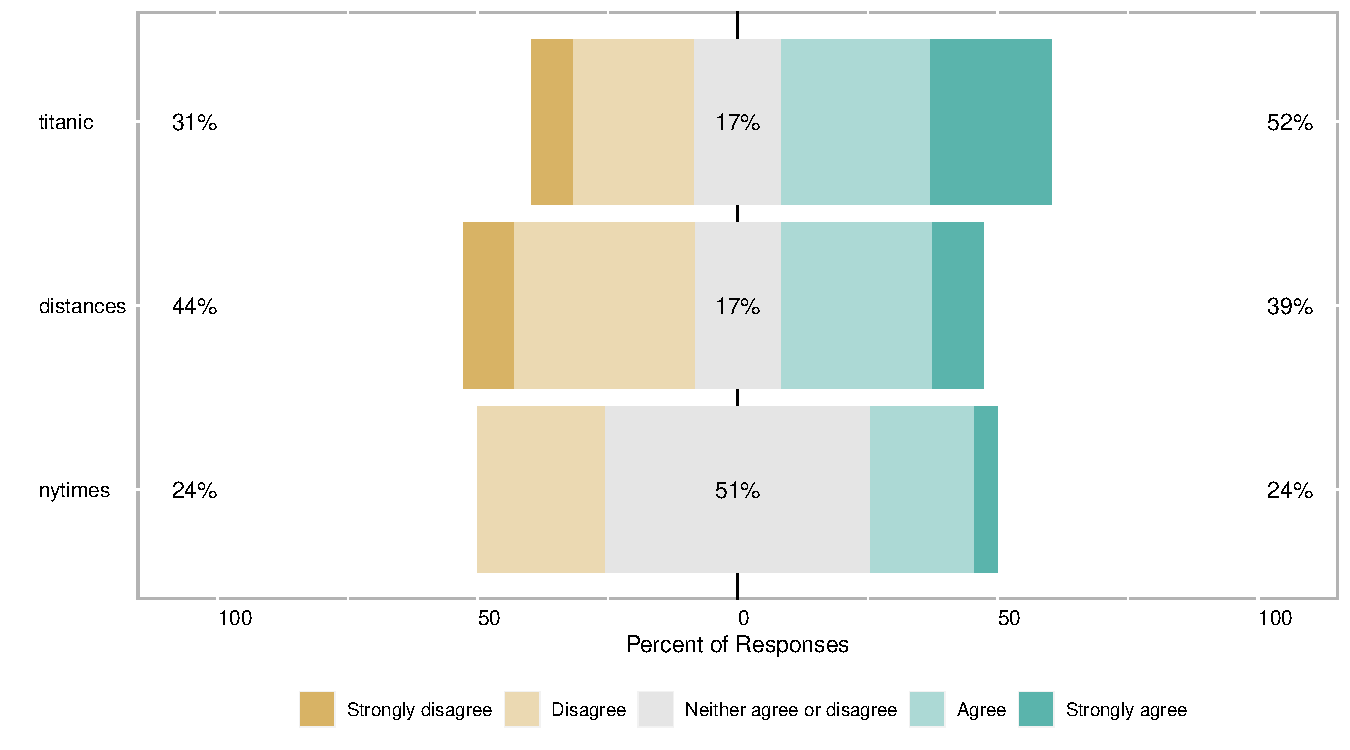
\includegraphics[width=.9\textwidth]{cp6/usefulness_overall.pdf}
    \caption{Diverging stacked plot of the usefulness of the text automatically identified for each task}
    \label{fig:usefulness-by-task}
\end{figure}





\begin{figure}[h!]
    \centering
    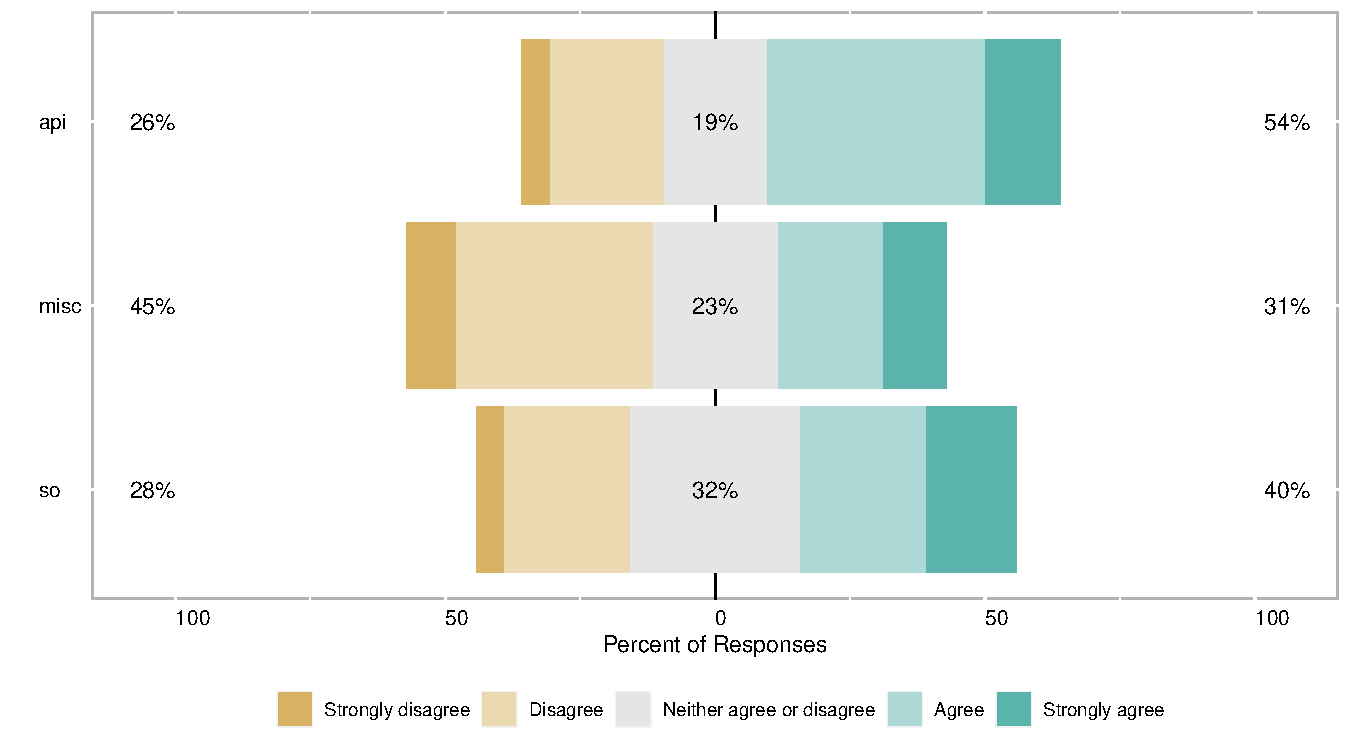
\includegraphics[width=.9\textwidth]{cp6/usefulness_per_type.pdf}
    \caption{Diverging stacked plot of the usefulness of the text automatically identified for each type of artifact}
    \label{fig:usefulness-by-artifact-type}
\end{figure}









